\subsection*{\lr{2.6.2} ساخت جدول معنایی \lr{(Construction of Semantic Tableaux)}}
  
  تجزیهٔ فرمول به مجموعه‌ای از \emph{لفظ‌ها} در قالب متنی دشوار است. در روش \emph{جدول معنایی}، مجموعه‌های فرمول برچسبِ گره‌های یک درخت را تشکیل می‌دهند، به‌طوری که هر مسیر در درخت نمایانگر فرمول‌هایی است که باید در یک تعبیر ممکن صدق‌پذیر شوند.
  
  \begin{itemize}
    \item فرمول اولیه برچسبِ ریشهٔ درخت است.
    \item هر گره، بسته به نوع فرمول برچسب‌خورده، یک یا دو فرزند دارد.
    \item برگ‌ها با مجموعه‌ای از \emph{لفظ‌ها} برچسب می‌خورند.
    \item برگ‌هایی که شامل یک \emph{زوج متمم از لفظ‌ها} باشند با «$\times$» (بسته) و برگ‌هایی که فاقد زوج متمم هستند با $\odot$ (باز) علامت‌گذاری می‌شوند.
  \end{itemize}
  
  شکل \lr{2.7} جدول‌های معنایی مثال‌های پیشین را نشان می‌دهد. جدول زیر نمونهٔ دیگری از جدول معنایی برای فرمول
  \[
  B = (p \lor q)\;\land\;(\neg p \land \neg q)
  \]
  را نمایش می‌دهد که ابتدا برای $p \lor q$ منشعب شده و سپس $\neg p \land \neg q$ را پردازش می‌کند. واضح است که اگر \emph{همگرایی} ($\land$) را پیش از \emph{جمع‌گزاره} ($\lor$) بگشاییم، تعداد گره‌ها کمتر خواهد بود و در نتیجه کارآمدتر است.
  
  \begin{figure}[ht]
    \centering
    \begin{latin}
      \resizebox{0.35\textwidth}{!}{
      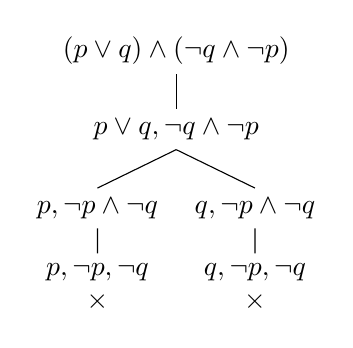
\begin{tikzpicture}[
        level distance=1cm,
        sibling distance=1.5cm,
        level 2/.style={sibling distance=2cm},
        level 2/.style={sibling distance=2cm},
        edge from parent path={(\tikzparentnode.south) -- (\tikzchildnode.north)}
      ]
      \node {$(p \lor q) \land (\neg q \land \neg p)$}
        child { 
          node {$p \lor q, \neg q \land \neg p$}
          child { 
            node {$p, \neg p \land \neg q$}
            child { node[align=center] {$p, \neg p, \neg q$ \\ $\times$} }
          }
          child { 
            node {$q, \neg p \land \neg q$}
            child { node[align=center] {$q, \neg p, \neg q$ \\ $\times$} }
          }
        };
      \end{tikzpicture}
      }
    \end{latin}
  \end{figure}
  
  برای ساده‌سازی و ایجاز، فرمول‌ها را بر اساس \emph{اپراتور اصلی} شان به دو دستهٔ \emph{$\alpha$-فرمول} و \emph{$\beta$-فرمول} تقسیم می‌کنیم (شکل \lr{2.8}):
  
  \begin{figure}[ht]
  \centering
  \begin{tabular}{|c|c|c|}
  \hline
  نوع & شکل عام & زیرفرمول‌ها \\
  \hline
  $\alpha$ & $A_1 \land A_2$ & $\alpha_1 = A_1,\;\alpha_2 = A_2$ \\
  $\alpha$ & $\neg(\neg A_1)$ & $\alpha_1 = A_1$ \\
  $\alpha$ & $\neg(A_1 \lor A_2)$ & $\alpha_1 = \neg A_1,\;\alpha_2 = \neg A_2$ \\
  $\alpha$ & $\neg(A_1 \to A_2)$ & $\alpha_1 = A_1,\;\alpha_2 = \neg A_2$ \\
  \hline
  $\beta$ & $A_1 \lor A_2$ & $\beta_1 = A_1,\;\beta_2 = A_2$ \\
  $\beta$ & $A_1 \to A_2$ & $\beta_1 = \neg A_1,\;\beta_2 = A_2$ \\
  $\beta$ & $\neg(A_1 \land A_2)$ & $\beta_1 = \neg A_1,\;\beta_2 = \neg A_2$ \\
  \hline
  \end{tabular}
  \renewcommand{\thefigure}{\lr{2.8}}
  \caption{طبقه‌بندی فرمول‌های آلفا و بتا}
  \end{figure}
  
  برای مثال، $p \land q$ یک $\alpha$-فرمول است (زیرا هر دو $p$ و $q$ باید صدق کنند)، و $\neg(p \land q)$ یک $\beta$-فرمول است (معادل $\neg p \lor \neg q$).
  
  \paragraph{\lr{2.64} الگوریتم ساخت جدول معنایی}
  \begin{enumerate}[1.]
    \item \textbf{ابتدایی‌سازی:}\\
      درختی با یک گرهٔ ریشه برچسب‌خورده $\phi$ بسازید. این گره هنوز علامت ندارد.
    \item \textbf{گسترش:}\\
      تا زمانی که برگ علامت‌نگرفته‌ای باقی بماند، مراحل زیر را تکرار کنید:
      \begin{enumerate}[a)]
        \item برگ $l$ را انتخاب کنید با مجموعهٔ برچسب $U(l)$ که هنوز علامت ندارد.
        \item اگر $U(l)$ \emph{مجموعه‌ای از لفظ‌ها} باشد:
          \begin{itemize}
            \item اگر شامل زوج متمم باشد، برگ را \emph{بسته} ($\times$) علامت بزنید.
            \item وگرنه، برگ را \emph{باز} ($\odot$) علامت بزنید.
          \end{itemize}
        \item در غیر این صورت (یعنی $U(l)$ شامل فرمول غیرلفظی است):
          \begin{enumerate}[(i]
            \item فرمولی $A\in U(l)$ را انتخاب کنید که \emph{لفظ} نباشد.
            \item بر اساس $\alpha$ یا $\beta$ بودن $A$ عمل کنید:
              \begin{itemize}
                \item \textbf{$\alpha$-فرمول:}\\
                  یک فرزند $l'$ بسازید با
                  \[
                  U(l') = \bigl(U(l) - \{A\}\bigr)\cup\{A_1,A_2\}.
                  \]
                  (اگر $A=\neg\neg A_1$ بود، تنها $\alpha_1$ را اضافه کنید.)
                \item \textbf{$\beta$-فرمول:}\\
                  دو فرزند $l'$ و $l''$ بسازید با
                  \[
                  U(l') = \bigl(U(l) - \{B\}\bigr)\cup\{B_1\},\quad
                  U(l'') = \bigl(U(l) - \{B\}\bigr)\cup\{B_2\}.
                  \]
              \end{itemize}
          \end{enumerate}
      \end{enumerate}
    \item \textbf{پایان:}\\
      وقتی هیچ برگ علامت‌نگرفته‌ای باقی نماند، الگوریتم تمام می‌شود.
  \end{enumerate}
  
  \begin{definition}[تعریف \lr{2.65}]
    \hfill
    \begin{itemize}
      \item جدولی که ساخت آن تکمیل شده، \emph{جدول تکمیل‌شده} نامیده می‌شود.
      \item یک جدول تکمیل‌شده \emph{بسته} است اگر \emph{همهٔ برگ‌ها} بسته ($\times$) باشند.
      \item در غیر این صورت (اگر دست‌کم یک برگ باز $\odot$ باشد)، جدول \emph{باز} است.
    \end{itemize}
  \end{definition}